\subsection{Attori}
\subsubsection{Attori Utenti}

\subsubsection{Attori Amministratori}
\begin{figure}[h]
  \caption{Gerarchia degli utenti}
  \centering
    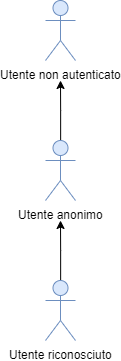
\includegraphics[scale=0.6]{sezioni/UseCase/Immagini/Utenti.png}
\end{figure}

\paragraph{Utente non autenticato}
Utente generico non ancora autenticato al sistema il quale ha una chiave LDPA ecc... non so sta cosa
\paragraph{Utente autenticato}
Utente generico che si è autenticato e che quindi dispone di credenziali (e-mail e password) per accedere all'applicazione.
\paragraph{Utente anonimo}
Utente autenticato non facente parte di alcuna organizzazione e quindi non rintracciabile all'interno di esse.

\paragraph{Utente riconosciuto}
Utente autenticato facente parte di una o più organizzazioni.
L'utente può venire monitorato quando è all'interno di esse.



\subsubsection{Attori Amministratori}
\begin{figure}[h]
  \caption{Gerarchia degli amministratori}
  \centering
    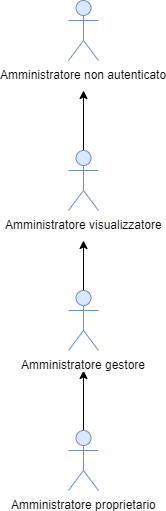
\includegraphics[scale=0.6]{sezioni/UseCase/Immagini/Amministratori.png}
\end{figure}


\paragraph{Amministratore non autenticato}
Amministratore generico non ancora autenticato al sistema il quale ha una chiave LDPA ecc... non so sta cosa
\paragraph{Amministratore autenticato}
Amministratore generico che si è autenticato al sistema
\paragraph{Amministratore organizzazione}
Amministratore autenticatosi con il ruolo di proprietario dell'organizzazione, il quale può compiere le seguenti funzioni:
\begin{itemize}
\item Gestire l'organizzazione
\item Gestire gli amministratori
\item Monitorare gli accessi
\item Eliminare l'organizzazione
\end{itemize}
Il proprietario dell'organizzazione può assumere altri amministratori.
\paragraph{Amministratore gestore}
Amministratore autenticatosi con il ruolo di gestore, il quale può compiere le seguenti funzioni:
\begin{itemize}
\item Gestire l'organizzazione
\item Monitorare gli accessi
\end{itemize}
\paragraph{Amministratore visualizzatore}
Amministratore autenticatosi con il ruolo di visualizzatore, il quale può compiere solo la seguente funzione:
\begin{itemize}
\item Monitorare gli accessi
\end{itemize}


